%% LyX 2.4.0~beta5 created this file.  For more info, see https://www.lyx.org/.
%% Do not edit unless you really know what you are doing.
\documentclass[english,footrule]{foils}
\usepackage[T1]{fontenc}
\usepackage[latin9]{inputenc}
\pagestyle{foilheadings}
\setcounter{secnumdepth}{1}
\setcounter{tocdepth}{1}
\usepackage{color}
\usepackage{pifont}
\usepackage{amsmath}
\usepackage{amsthm}
\usepackage{amssymb}
\usepackage{graphicx}

\makeatletter

%%%%%%%%%%%%%%%%%%%%%%%%%%%%%% LyX specific LaTeX commands.
%% A simple dot to overcome graphicx limitations
\newcommand{\lyxdot}{.}


%%%%%%%%%%%%%%%%%%%%%%%%%%%%%% Textclass specific LaTeX commands.
\newenvironment{lyxcode}
	{\par\begin{list}{}{
		\setlength{\rightmargin}{\leftmargin}
		\setlength{\listparindent}{0pt}% needed for AMS classes
		\raggedright
		\setlength{\itemsep}{0pt}
		\setlength{\parsep}{0pt}
		\normalfont\ttfamily}%
	 \item[]}
	{\end{list}}

%%%%%%%%%%%%%%%%%%%%%%%%%%%%%% User specified LaTeX commands.
\newcommand{\argmin}{\operatornamewithlimits{argmin}}

\usepackage{xcolor}
\renewcommand{\labelitemi}{$\textcolor{blue}{\bullet}$}
\renewcommand{\labelitemii}{$\textcolor{teal}{\Rightarrow}$}
\renewcommand{\labelitemiii}{$\textcolor{red}{\rightarrow}$}
\renewcommand{\labelitemiv}{$\textcolor{brown}{\circ}$}

\newcommand{\T}{\mathrm{T}}  % transpose
\newcommand{\PP}{\mathrm{P}}  % probability
\newcommand{\dd}{\mathrm{d}} % integration dx
\newcommand{\ee}{\mathrm{e}} % exponential
\newcommand{\E}{\mathrm{E}} % expectation

\makeatother

\usepackage{babel}
\begin{document}

\MyLogo{Intro ML--Clustering Analysis}
\title{Unsupervised Learning - Clustering\\
\rule[0.5ex]{1\columnwidth}{3pt}}
\author{Mark Asch - IMU/VLP/CSU }
\date{2023}
\maketitle

\foilhead{Program}
\begin{enumerate}
\item Data Analysis

\begin{enumerate}
\item Introduction: the 4 identifiers of ``big data'' and ``data science''
\item Supervised learning methods: regression---advanced, k-NN, linear
classification methods, SVM, NN, decision trees. 
\item \textcolor{red}{Unsupervised learning methods}: principal component
analysis, \textcolor{red}{k-means, clustering}.
\end{enumerate}
\end{enumerate}

\foilhead{Recall: Introduction}
\begin{itemize}
\item \textcolor{magenta}{Supervised} learning: 

\begin{itemize}
\item we have $p$ characteristics $X_{1},X_{2},\ldots,X_{p}$ measured
on $n$ observations 
\item one response $Y$ measured on the same observations
\item objective: predict $Y$ using $X_{1},X_{2},\ldots,X_{p}$
\item methods: regression and classification
\end{itemize}
\item \textcolor{magenta}{Unsupervised} learning: 

\begin{itemize}
\item we \textcolor{magenta}{only }have $p$ characteristics $X_{1},X_{2},\ldots,X_{p}$
measured on $n$ observations 
\item we want to make predictions, but we do not have an associated response
variable...
\item objective: \textcolor{magenta}{discover interesting effects} with
respect to the observations of $X_{1},X_{2},\ldots,X_{p}$ 

\begin{itemize}
\item Can we\textcolor{magenta}{{} visualize }or represent the data in a more
\textcolor{magenta}{informative} way? 
\item Can we \textcolor{magenta}{discover sub-groups or clusters} among
the variables or the observations? 
\end{itemize}
\end{itemize}
\end{itemize}

\foilhead{Recall: Warnings!}
\begin{itemize}
\item Unsupervised learning is more difficult, since it is subjective.
\end{itemize}
\begin{dinglist}{56}
\item Unsupervised learning is often part of an initial phase of \textcolor{magenta}{exploratory
data analysis} (EDA), where we compute elementary statistics and plot
basic histograms and boxplots-{}-{}-see Introductory lectures.
\item There are no universal \textcolor{magenta}{cross-validation} methods
for unsupervised learning. 
\item There is \textcolor{magenta}{no response variable} that can be used
to test our models.
\end{dinglist}
\begin{dinglist}{52}
\item However, there are a large number of application domains where unsupervised
learning is widely used.
\end{dinglist}

\foilhead[-0.5in]{Introduction to Clustering}
\begin{itemize}
\item Clustering is an ensemble of methods for finding subgroups, or clusters,
in a database. 
\item The subgroups are defined according to two principles:
\begin{itemize}
\item The observations within each group are \textcolor{magenta}{similar}. 
\item The observations in different groups are \textcolor{magenta}{different}. 
\end{itemize}
\item For example, suppose we have $n$ observations, each with $p$ properties. 
\begin{itemize}
\item The properties correspond to \textcolor{magenta}{measurements} made
for each sample among the $n$. 
\item The clustering will enable us to distinguish between \textcolor{magenta}{subtypes}
within the measurements 
\item The problem is \textcolor{magenta}{unsupervised} because we are attempting
to discover the unknown structure, based exclusively on the measured
data.
\end{itemize}
\end{itemize}

\foilhead{Clustering Approaches}

There are a large number of clustering methods. The two best known
are: 
\begin{enumerate}
\item $k$-means clustering. 
\item Hierarchical, or tree clustering. 
\end{enumerate}
The major difference is that: 
\begin{itemize}
\item in $k$-means we try to divide the observations into a \textcolor{magenta}{specified
}number of clusters, 
\item whereas in the hierarchical approach we do not know in advance the
number of clusters, and we end up with a tree-like structure known
as a \textcolor{magenta}{dendrogram}. This structure enables us to
visualize all the possible clusterings, from $1$ to $n.$
\item \textbf{Note}:
\begin{itemize}
\item both PCA and clustering seek to simplify the data by means of a small
number of parameters, but their \textcolor{magenta}{mechanisms} are
different:
\item PCA tries to find a \textcolor{magenta}{low dimensional representation}
of the observations that explains a large proportion of the variance. 
\item Clustering tries to find \textcolor{magenta}{homogeneous subgroups}
among the observations. 
\end{itemize}
\end{itemize}

\foilhead{$\;$}

\vfill{}

\begin{center}
{\Large\textbf{\textcolor{blue}{K-MEANS CLUSTERING}}}{\Large\par}
\par\end{center}

\vfill{}


\foilhead{k-means Clustering}
\begin{itemize}
\item This is a simple and elegant method for dividing a dataset into $k$
\textcolor{magenta}{distinct clusters }with no overlaps. 
\item To do the clustering, one must first specify the \textcolor{magenta}{number
of desired clusters}, $K.$ 
\item The algorithm will then \textcolor{magenta}{assign} each observation
to at most one of the $K$ clusters. 
\begin{itemize}
\item Since we do not know the value of $k,$ the algorithm will be based
on an optimization problem.
\end{itemize}
\end{itemize}
\begin{figure}
\begin{centering}
\includegraphics[scale=0.6]{\string"/Users/markasch/Dropbox/3Teaching/stat-ML/M2/03resources/ISLR/All Figures/Chapter10/10.5\string".png}
\par\end{centering}
\caption{Application of k-means to simulated 2-D data.}
\end{figure}


\foilhead[-0.5in]{Theory of k-means}
\begin{itemize}
\item Let $C_{1},\ldots,C_{K}$ be the sets containing the indices of the
observations in each of the $K$ clusters. 
\item These sets satisfy two properties:
\begin{enumerate}
\item $C_{1}\cup C_{2}\cup\cdots\cup C_{K}=\left\{ 1,\ldots,n\right\} ,$
so each observation belongs to at least one of the $K$ clusters. 
\item $C_{k}\cap C_{k'}=\emptyset$ for all $k\neq k',$ meaning that the
clusters do not overlap and no observation can belong to more than
one cluster. 
\end{enumerate}
\item Then a ``good'' clustering is defined as one for which the intra-cluster
variation, $W(C_{k}),$ is the smallest possible. That is, we want
to solve the optimization problem 
\[
\min_{C_{1},\ldots,C_{K}}\left\{ \sum_{k=1}^{K}W(C_{k})\right\} ,
\]
with a suitable definition of the variation $W(C_{k}).$ 
\item There are several possibilities for this, but we usually just use
the\textcolor{magenta}{{} squared Euclidean distance}, 
\[
W(C_{k})=\frac{1}{\left|C_{k}\right|}\sum_{i,i'\in C_{k}}\sum_{j=1}^{p}\left(x_{ij}-x_{i'j}\right)^{2},
\]
where $\left|C_{k}\right|$ is the number of observations in the $k$-th
cluster. 
\item Substituting this expression, we obtain the $k$-means \textcolor{magenta}{optimization}
problem, 
\begin{equation}
\min_{C_{1},\ldots,C_{K}}\left\{ \sum_{k=1}^{K}\frac{1}{\left|C_{k}\right|}\sum_{i,i'\in C_{k}}\sum_{j=1}^{p}\left(x_{ij}-x_{i'j}\right)^{2}\right\} .\label{eq:k-means-cost}
\end{equation}
\end{itemize}

\foilhead[-0.5in]{Algorithm for k-means}
\begin{itemize}
\item Solving this optimization problem is not trivial. 
\begin{itemize}
\item How do we find a division of the observations into $K$ clusters that
guarantees the minimization of the above cost function? 
\end{itemize}
\item It can be proved that a very simple algorithm can find an acceptable
solution.

\begin{itemize}
\item (1) Assign a number between $1$ and $K$ at \textcolor{magenta}{random}
to each observation-{}-this produces the initial clustering.
\item (2) Iterate the following until the cluster assignments do not change
anymore: 
\begin{itemize}
\item (2a) For each cluster, \textcolor{magenta}{compute the centroid }equal
to the vector of the $p$ characteristic means for all observations
in cluster $p.$
\item (2b)\textcolor{magenta}{{} Assign} each observation to the cluster whose
centroid is closest as defined by the chosen distance function.
\end{itemize}
\end{itemize}
\end{itemize}
\begin{figure}
\begin{centering}
\includegraphics[width=1\textwidth]{\string"/Users/markasch/Dropbox/3Teaching/stat-ML/M2/03resources/ISLR/All Figures/Chapter10/10.6\string".pdf}
\par\end{centering}
\caption{Progress of the k-means algorithm}
\end{figure}

\begin{dinglist}{52}
\item Since this algorithm finds a \textcolor{magenta}{local optimum}, the
results will depend on the initial, random assignment of labels. 
\begin{dinglist}{52}
\item It is thus vital to \textcolor{magenta}{relaunch} the algorithm a
large number of times, starting from different random initial configurations. 
\item Finally, we choose the \textcolor{magenta}{best solution} that produces
the smallest value of the cost function.
\end{dinglist}
\end{dinglist}

\foilhead[-0.5in]{~}

\begin{figure}
\begin{centering}
\includegraphics[width=1\textwidth]{\string"/Users/markasch/Dropbox/3Teaching/stat-ML/M2/03resources/ISLR/All Figures/Chapter10/10_7\string".pdf}
\par\end{centering}
\caption{Six runs with $K=3$}
\end{figure}


\foilhead[-0.5in]{Practical Considerations for Clustering}
\begin{itemize}
\item Clustering is a very useful tool for data analysis. 
\item Before starting, we must make two decisions whose potential impacts
are fundamental:
\begin{enumerate}
\item Should we normalize (center and reduce) the attributes? 
\item How many clusters should we seek? 
\end{enumerate}
\item In practice we will have to try several options, since there is no
single answer to these two questions. 
\item The problem of validating the computed clusters is a subject of ongoing
research. 
\item Finally, to interpret the results, one can do the following:
\begin{itemize}
\item Tune the parameters---see Examples below. 
\item Check the robustness by recalculating over subsets of the data---a
form of cross-validation. 
\item Be very cautious when reporting the results---they do not represent
the absolute truth! 
\end{itemize}
\end{itemize}

\foilhead[-0.5in]{Example}
\begin{itemize}
\item The function \texttt{\textcolor{blue}{kmeans()}} performs k-means
clustering in \texttt{\textcolor{blue}{R}}
\item Consider a simple, simulated example: there are 2 clusters in the
data, with a shift in their mean values between the first 25 and the
last 25 observations
\end{itemize}
\begin{lyxcode}
set.seed(2)~

x=matrix(rnorm(50{*}2),~ncol=2)~

x{[}1:25,1{]}=x{[}1:25,1{]}+3~

x{[}1:25,2{]}=x{[}1:25,2{]}-4

head(x)

\#\#~~~~~~~~~~{[},1{]}~~~~~~{[},2{]}~

\#\#~{[}1,{]}~2.103085~-4.838287~

\#\#~{[}2,{]}~3.184849~-1.933699~

\#\#~{[}3,{]}~4.587845~-4.562247~

\#\#~{[}4,{]}~1.869624~-2.724284~

\#\#~{[}5,{]}~2.919748~-5.047573~

\#\#~{[}6,{]}~3.132420~-5.965878
\end{lyxcode}
\begin{itemize}
\item First, perform k-means with $K=2$ :
\end{itemize}
\begin{lyxcode}
km.out=kmeans(x,2,nstart=20)~
\end{lyxcode}
\begin{itemize}
\item The affectations of the observations are in the variable \texttt{cluster}:
\end{itemize}
\begin{lyxcode}
km.out\$cluster~

\#\#~~{[}1{]}~2~2~2~2~2~2~2~2~2~2~2~2~2~2~2~

~~~~~~~~2~2~2~2~2~2~2~2~2~2~1~1~1~1~1~

~~~~~~~~1~1~1~1~1~

\#\#~{[}36{]}~1~1~1~1~1~1~1~1~1~1~1~1~1~1~1
\end{lyxcode}
\begin{itemize}
\item We observe that k-means has perfectly separated the observations into
two clusters, without us having supplied any group information to
\texttt{\textcolor{blue}{kmeans()...}}
\item Plot the observations, colored by their cluster affectation :
\end{itemize}
\begin{lyxcode}
{\small plot(x,~col=(km.out\$cluster+1),~main=\textquotedbl k-Means~Clustering~}{\small\par}

{\small ~~~~Results~with~K=2\textquotedbl ,~xlab=\textquotedbl\textquotedbl ,~ylab=\textquotedbl\textquotedbl ,~pch=20,~cex=2)~}{\small\par}

\includegraphics[width=0.8\textwidth]{/Users/markasch/Dropbox/6Books/DTbook/src/codes/k-means/k-means-simple_files/figure-latex/unnamed-chunk-4-1}
\end{lyxcode}
\begin{itemize}
\item Here, the observations are easy to plot, since we are in 2 dimensions
only... In the case of more than 2 variables, we could perform a PCA
and then plot the first 2 principal components.
\item In this simulated example we knew the number of clusters. But in general
this is definitely not the case. So we could have started by trying
$K=3$ : 
\end{itemize}
\begin{lyxcode}
set.seed(4)~

km.out=kmeans(x,3,nstart=20)~

km.out~

{\small plot(x,~col=(km.out\$cluster+1),~main=\textquotedbl K-Means~Clustering~}{\small\par}

{\small Results~with~K=3\textquotedbl ,~xlab=\textquotedbl\textquotedbl ,~ylab=\textquotedbl\textquotedbl ,~pch=20,~cex=2)~}{\small\par}

{\footnotesize\#\#~K-means~clustering~with~3~clusters~of~sizes~10,~23,~17~}{\footnotesize\par}

{\footnotesize\#\#~~}{\footnotesize\par}

{\footnotesize\#\#~Cluster~means:~}{\footnotesize\par}

{\footnotesize\#\#~~~~~~~~~{[},1{]}~~~~~~~~{[},2{]}~}{\footnotesize\par}

{\footnotesize\#\#~1~~2.3001545~-2.69622023~}{\footnotesize\par}

{\footnotesize\#\#~2~-0.3820397~-0.08740753~}{\footnotesize\par}

{\footnotesize\#\#~3~~3.7789567~-4.56200798~}{\footnotesize\par}

{\footnotesize\#\#~~}{\footnotesize\par}

{\footnotesize\#\#~Clustering~vector:~}{\footnotesize\par}

{\footnotesize\#\#~~{[}1{]}~3~1~3~1~3~3~3~1~3~1~3~1~3~1~3~1~3~3~3~3~3~1~3~3~3~}{\footnotesize\par}

{\footnotesize ~~~~~~~~2~2~2~2~2~2~2~2~2~2~}{\footnotesize\par}

{\footnotesize\#\#~{[}36{]}~2~2~2~2~2~2~2~2~1~2~1~2~2~2~2~}{\footnotesize\par}

{\footnotesize\#\#~~}{\footnotesize\par}

{\footnotesize\#\#~Within~cluster~sum~of~squares~by~cluster:~}{\footnotesize\par}

{\footnotesize\#\#~{[}1{]}~19.56137~52.67700~25.74089~}{\footnotesize\par}

{\footnotesize\#\#~~(between\_SS~/~total\_SS~=~~79.3~\%)~}{\footnotesize\par}

{\footnotesize\#\#~~}{\footnotesize\par}

{\footnotesize\#\#~Available~components:~}{\footnotesize\par}

{\footnotesize\#\#~~}{\footnotesize\par}

{\footnotesize\#\#~{[}1{]}~\textquotedbl cluster\textquotedbl ~~~~~~\textquotedbl centers\textquotedbl ~~~~~~\textquotedbl totss\textquotedbl ~~~~~~~~\textquotedbl withinss\textquotedbl ~~~~~}{\footnotesize\par}

{\footnotesize\#\#~{[}5{]}~\textquotedbl tot.withinss\textquotedbl ~\textquotedbl betweenss\textquotedbl ~~~~\textquotedbl size\textquotedbl ~~~~~~~~~\textquotedbl iter\textquotedbl ~~~~~~~~~}{\footnotesize\par}

{\footnotesize\#\#~{[}9{]}~\textquotedbl ifault\textquotedbl}{\footnotesize\par}

\includegraphics[width=0.8\textwidth]{/Users/markasch/Dropbox/6Books/DTbook/src/codes/k-means/k-means-simple_files/figure-latex/unnamed-chunk-5-1}
\end{lyxcode}
\begin{itemize}
\item Here, the algorithm has divided one of the original 2 clusters...
\item Note that to execute \texttt{\textcolor{blue}{kmeans()}} with different
initial affectations, we use the argument \texttt{\textcolor{blue}{nstart}}.
here we compare \texttt{\textcolor{blue}{nstart=1}} with \texttt{\textcolor{blue}{nstart=20}}
by extracting the intracluster sum of squares score.
\end{itemize}
\begin{lyxcode}
set.seed(3)~

km.out=kmeans(x,3,nstart=1)~

km.out\$tot.withinss~

\#\#~{[}1{]}~104.3319

km.out=kmeans(x,3,nstart=20)~

km.out\$tot.withinss

\#\#~{[}1{]}~97.97927~
\end{lyxcode}
\begin{itemize}
\item \textbf{Conclusions}:
\begin{itemize}
\item Restarting has effectively reduced the value of the intracluster sum
of squares.
\item We have attained a better optimum (minimum).
\end{itemize}
\item It is strongly recommended to execute many times, using a high value
of\texttt{\textcolor{blue}{{} nstart}}, such as 20 or 50, otherwise
undesirable local minima will be found...
\item We also use a random seed initialization, by \texttt{\textcolor{blue}{set.seed(),}}
to ensure reproducibility of the results.
\end{itemize}

\foilhead{$\;$}

\vfill{}

\begin{center}
{\Large\textbf{\textcolor{blue}{HIERARCHICAL CLUSTERING}}}{\Large\par}
\par\end{center}

\vfill{}


\foilhead{Hierarchical Clustering }
\begin{itemize}
\item No need to choose the number of clusters \textcolor{magenta}{beforehand}.
\item Everything is done `` \textcolor{magenta}{bottom-up},'' starting from
the leaves and moving up to the trunk, or main branch
\item This generates a tree-like diagram, known as a \textcolor{magenta}{dendrogram}.
\item It is a \textcolor{magenta}{deterministic} method, but can provide
clues for further inference in statistical models.
\end{itemize}

\foilhead{Interpretation}
\begin{itemize}
\item Suppose we have synthetic data, in 2D, having 3 distinct classes,
but that are observed WITHOUT any knowledge of their classes.
\end{itemize}
\begin{figure}
\begin{centering}
\includegraphics[scale=0.8]{\string"/Users/markasch/Dropbox/3Teaching/stat-ML/M2/03resources/ISLR/All Figures/Chapter10/10.8\string".pdf}
\par\end{centering}
\caption{45 observations in 3 classes}
\end{figure}

\begin{figure}
\begin{centering}
\includegraphics[scale=0.8]{\string"/Users/markasch/Dropbox/3Teaching/stat-ML/M2/03resources/ISLR/All Figures/Chapter10/10.9\string".png}
\par\end{centering}
\caption{Dendrogram obtained by hierarchical clustering with full linkage.}
\end{figure}

\begin{itemize}
\item Each leaf represents one of the 45 observations (figure on left).
\item Moving up, the leaves merge into branches, corresponding to observations
that have a similarity-{}-{}-measured in a given metric-{}-{}-between
them.
\begin{itemize}
\item The earlier the merging takes place, the more similar are the observations.
\item Thus, observations that merge later-{}-{}-towards the top-{}-{}-are
more and more different.
\end{itemize}
\item Conclusion: the merging \textcolor{magenta}{height}, on the vertical
axis, indicates the difference between two observations and it is
the height that will determine the number of different clusters.
\item Identification of clusters: 
\begin{itemize}
\item make a horizontal cut across the dendrogram
\item the distinct sets below can be interpreted as distinct clusters
\item further cuts can be made, going downwards, until each observation
is in its own cluster... (this is not very useful!)
\end{itemize}
\item A single dendrogram can provide any number of clusters, from $1$
to $N,$ the number of observations.
\begin{itemize}
\item Choosing the ``good'' number of clusters, or cut height, is not an
obvious task, and has to be performed visually, based on experience,
or familiarity with the data
\item Hopefully, however, there is a clear gap in the link lengths of the
dendrogram that will separate the \textcolor{magenta}{inherent} clusters
from the unnatural ones. This will depend on the context and the data.
\end{itemize}
\item The dendrogram does not work better than K-means, unless the data
are truly hierarchical... (without other divisions, eg. male-female)
\end{itemize}

\foilhead{Algorithm for hierarchical clustering }
\begin{enumerate}
\item For all $n$ observations, calculate the $n(n-1)/2$ dissimilarities
pairwise. Each observation is a cluster.
\item For $i=n,n-1,\ldots,2,$ 
\begin{enumerate}
\item calculate all the inter-cluster dissimilarities and identify the pair
of two clusters that are the least dissimilar
\item merge these two clusters where the dissimilarity indicates the height
in the dendrogram at which the merge takes place
\item calculate the new inter-cluster dissimilarities among the remaining
$i-1$ clusters
\end{enumerate}
\end{enumerate}

\foilhead{Dissimilarity between 2 groups}
\begin{itemize}
\item Need to generalize the notion of dissimilarity between a pair of observations,
to the dissimilarity between a pair of groups (inter-cluster).
\item We use the notion of \textcolor{magenta}{linkage} that defines the
dissimilarity between 2 groups of observations.
\end{itemize}
\includegraphics[width=0.9\textwidth]{/Users/markasch/Dropbox/3Teaching/stat-ML/01Common/01Lessons/graphics/Different-linkage-methods-for-hierarchical-clustering_W640.jpeg}
\begin{itemize}
\item Four types of linkage :
\begin{itemize}
\item complete
\item average
\item single
\item centroid
\end{itemize}
\item We usually choose \textcolor{magenta}{complete} or \textcolor{magenta}{average},
since they produce more balanced dendrograms.
\item Centroid is often used in genomics.
\end{itemize}

\foilhead{Further indications}
\begin{itemize}
\item For the dissimilarity between 2 observations, we use:
\begin{itemize}
\item Euclidean distance (most used)
\item Correlation distance
\end{itemize}
\item The choice of this distance is very important, and is context-dependent.
\item Scaling: as for k-means, we must pay attention to the context.
\item It is strongly recommended to test several choices of:
\begin{itemize}
\item distance
\item linkage
\item cut height
\end{itemize}
\end{itemize}

\foilhead{Example}
\begin{itemize}
\item The function\texttt{\textcolor{blue}{{} hclust()}} performs hierarchical
clustering in \textcolor{blue}{R}.
\item Take the following simulated data :
\end{itemize}
\begin{lyxcode}
set.seed~(222)~

x=matrix~(rnorm~(50{*}2)~,~ncol~=2)~

x{[}1:25~,1{]}~=~x{[}1:25~,1{]}~+~3~

x{[}1:25~,2{]}~=~x{[}1:25~,2{]}~-~4~

head(x)

\#\#~~~~~~~~~{[},1{]}~~~~~~{[},2{]}~

\#\#~{[}1,{]}~4.487757~-3.405585~

\#\#~{[}2,{]}~2.998108~-3.479132~

\#\#~{[}3,{]}~4.381021~-4.952044~

\#\#~{[}4,{]}~2.619786~-5.227685~

\#\#~{[}5,{]}~3.184136~-4.202407~

\#\#~{[}6,{]}~2.753104~-2.940880~
\end{lyxcode}
\begin{itemize}
\item Use the Euclidean distance to compute the clusterings with complete,
average and single linkages.
\end{itemize}
\begin{lyxcode}
hc.complete~=~hclust(dist(x),~method=\textquotedbl complete\textquotedbl )~

hc.average~~=~hclust(dist(x),~method=\textquotedbl average\textquotedbl )~

hc.single~~~=~hclust(dist(x),~method=\textquotedbl single\textquotedbl )
\end{lyxcode}
\begin{itemize}
\item Plot the dendrograms. 
\end{itemize}
\begin{lyxcode}
{\footnotesize par(mfrow=c(1,3))~}{\footnotesize\par}

{\footnotesize plot(hc.complete,main=\textquotedbl Complete~Linkage\textquotedbl ,~xlab=\textquotedbl\textquotedbl ,~sub=\textquotedbl\textquotedbl ,~cex=.9)~}{\footnotesize\par}

{\footnotesize plot(hc.average,~main=\textquotedbl Average~Linkage\textquotedbl ,~xlab=\textquotedbl\textquotedbl ,~sub=\textquotedbl\textquotedbl ,~cex=.9)~}{\footnotesize\par}

{\footnotesize plot(hc.single,~main=\textquotedbl Single~Linkage\textquotedbl ,~xlab=\textquotedbl\textquotedbl ,~sub=\textquotedbl\textquotedbl ,~cex=.9)}{\footnotesize\par}

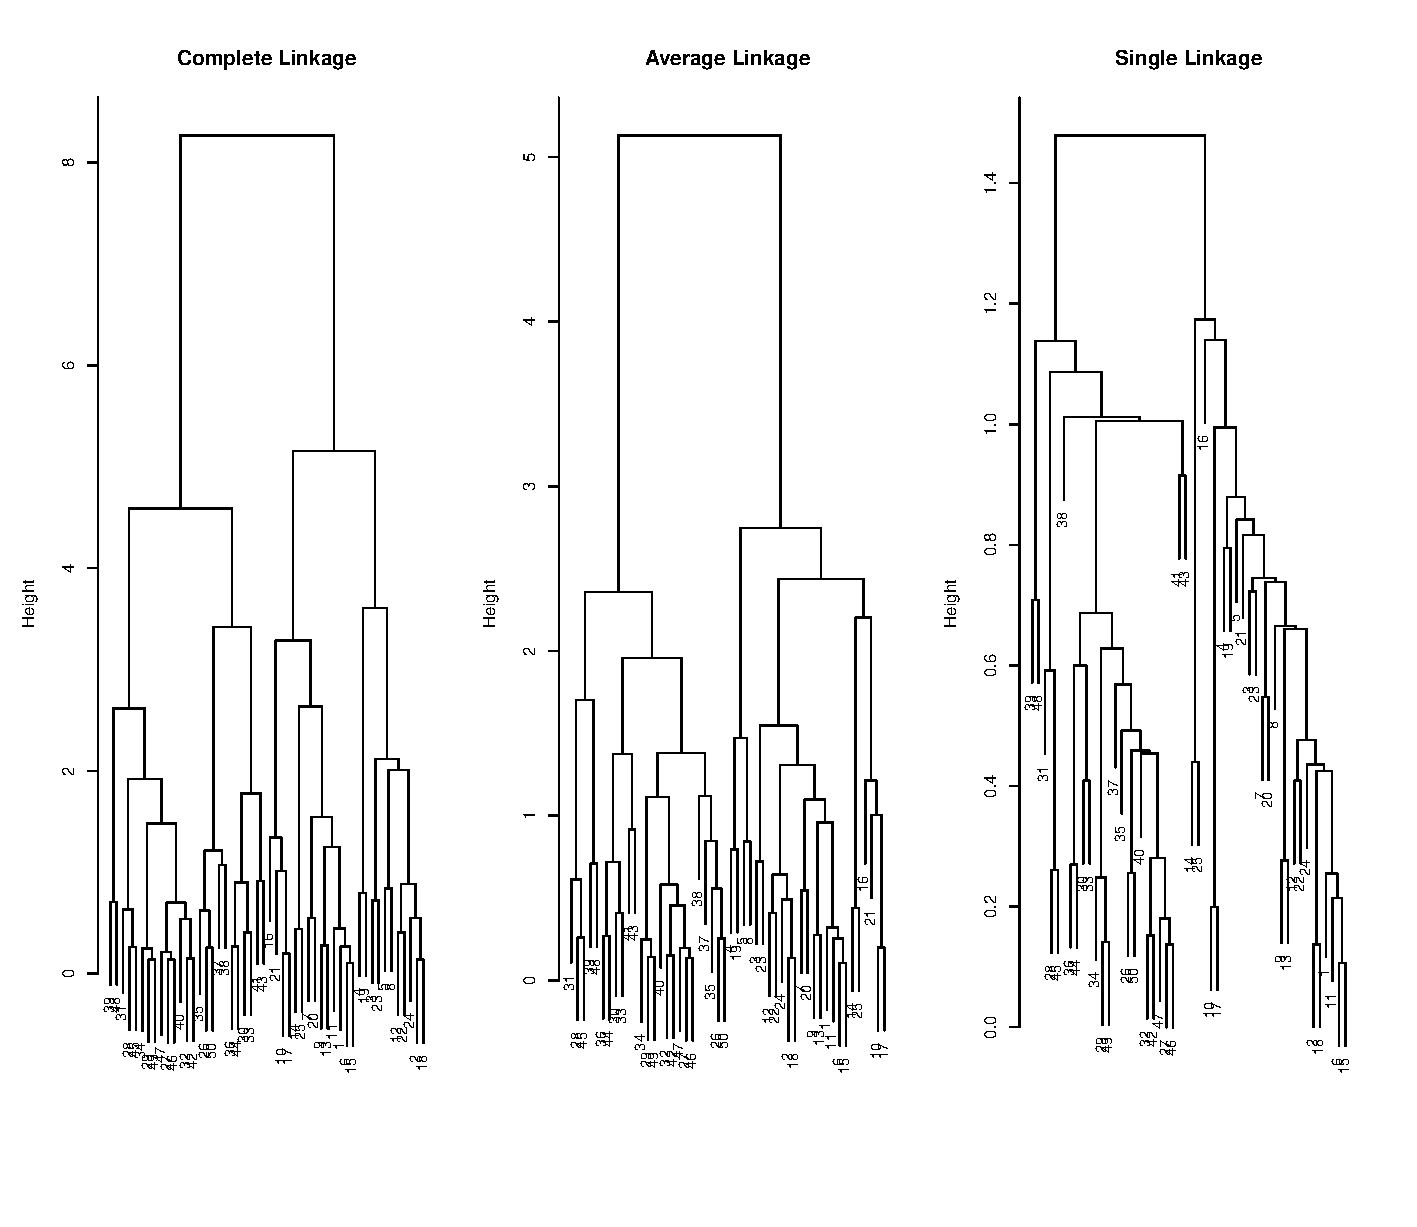
\includegraphics[scale=0.55]{graphics/dendro-1}
\end{lyxcode}
\begin{itemize}
\item Display the cluster labels for each observation associated with a
given cut
\end{itemize}
\begin{lyxcode}
cutree(hc.complete,~2)~

{\footnotesize{[}1{]}~1~1~1~1~1~1~1~1~1~1~1~1~1~1~1~1~1~1~1~1~1~1~1~1~1~2~2~2~2}{\footnotesize\par}

{\footnotesize{[}30{]}~2~2~2~2~2~2~2~2~2~2~2~2~2~2~2~2~2~2~2~2~2}{\footnotesize\par}

cutree(hc.average,~2)

{\footnotesize{[}1{]}~1~1~1~1~1~1~1~1~1~1~1~1~1~1~1~1~1~1~1~1~1~1~1~1~1~2~2~2~2~}{\footnotesize\par}

{\footnotesize{[}30{]}~2~2~2~1~2~2~2~2~2~2~2~2~2~2~1~2~1~2~2~2~2}{\footnotesize\par}

cutree(hc.single,~2)

{\footnotesize{[}1{]}~1~1~1~1~1~1~1~1~1~1~1~1~1~1~1~2~1~1~1~1~1~1~1~1~1~1~1~1~1}{\footnotesize\par}

{\footnotesize{[}30{]}~1~1~1~1~1~1~1~1~1~1~1~1~1~1~1~1~1~1~1~1~1}{\footnotesize\par}
\end{lyxcode}
\begin{itemize}
\item The complete and average linkages give good results, but the simple
is not accurate.
\item For scaling, we can use the function \texttt{\textcolor{blue}{scale()}}
\end{itemize}
\begin{lyxcode}
{\footnotesize xsc=scale(x)~}{\footnotesize\par}

{\footnotesize plot(hclust(dist(xsc),~method=\textquotedbl complete\textquotedbl ),~}{\footnotesize\par}

{\footnotesize ~~~main=\textquotedbl Hierarchical~Clustering~with~Scaled~Features\textquotedbl )~}{\footnotesize\par}

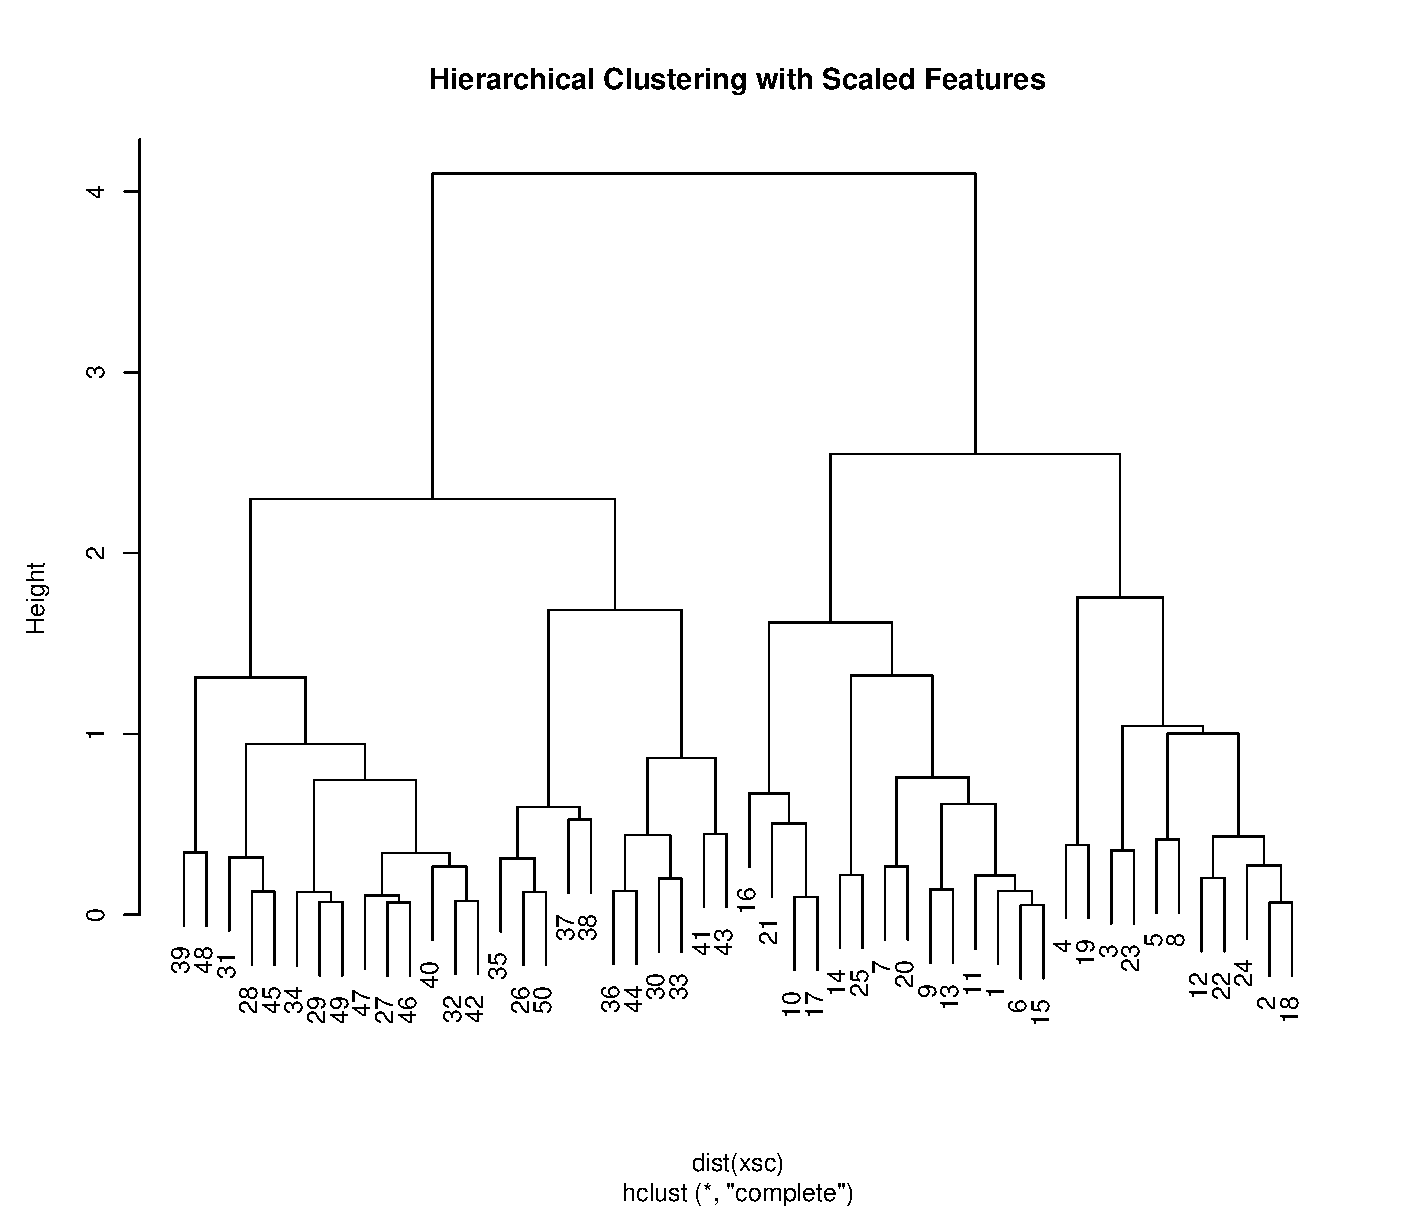
\includegraphics[scale=0.6]{graphics/dendro-2}
\end{lyxcode}

\foilhead{References}
\begin{enumerate}
\item M. DeGroot, M. Schervish, \emph{Probability and Statistics}, Addison
Wesley, 2002.
\item Spiegel, Murray and Larry Stephens,\emph{ Schaum's Outline of Statistics,}
6th edition, McGraw Hill. 2017.
\item G. James, D. Witten, T. Hastie, R. Tibshirani. \emph{An Introduction
to Statistical Learning with Applications in R.} Springer. 2013.
\item T. Hastie, R. Tibshirani, J. Friedman. \emph{The Elements of Statistical
Learning}. Springer. 2009.
\item Rachel Schutt and Cathy O\textquoteright Neil. \emph{Doing Data Science.}
O'Reilly. 2014.
\end{enumerate}

\end{document}
